%%%%%%%%%%%%%%%%%%%%%%%%%%%%%%%%%%%%%%%%%
% Masters/Doctoral Thesis 
% LaTeX Template
% Version 2.5 (27/8/17)
%
% This template was downloaded from:
% http://www.LaTeXTemplates.com
%
% Version 2.x major modifications by:
% Vel (vel@latextemplates.com)
%
% This template is based on a template by:
% Steve Gunn (http://users.ecs.soton.ac.uk/srg/softwaretools/document/templates/)
% Sunil Patel (http://www.sunilpatel.co.uk/thesis-template/)
%
% Template license:
% CC BY-NC-SA 3.0 (http://creativecommons.org/licenses/by-nc-sa/3.0/)
%
%%%%%%%%%%%%%%%%%%%%%%%%%%%%%%%%%%%%%%%%%

%----------------------------------------------------------------------------------------
%	PACKAGES AND OTHER DOCUMENT CONFIGURATIONS
%----------------------------------------------------------------------------------------

\documentclass[
11pt, % The default document font size, options: 10pt, 11pt, 12pt
oneside, % Two side (alternating margins) for binding by default, uncomment to switch to one side
english, % ngerman for German
singlespacing, % Single line spacing, alternatives: onehalfspacing or doublespacing
%draft, % Uncomment to enable draft mode (no pictures, no links, overfull hboxes indicated)
%nolistspacing, % If the document is onehalfspacing or doublespacing, uncomment this to set spacing in lists to single
%liststotoc, % Uncomment to add the list of figures/tables/etc to the table of contents
%toctotoc, % Uncomment to add the main table of contents to the table of contents
%parskip, % Uncomment to add space between paragraphs
%nohyperref, % Uncomment to not load the hyperref package
headsepline, % Uncomment to get a line under the header
%chapterinoneline, % Uncomment to place the chapter title next to the number on one line
%consistentlayout, % Uncomment to change the layout of the declaration, abstract and acknowledgements pages to match the default layout
]{MastersDoctoralThesis} % The class file specifying the document structure

\usepackage[utf8]{inputenc} % Required for inputting international characters
\usepackage[T1]{fontenc} % Output font encoding for international characters
\usepackage{amsmath}
\usepackage{graphicx}

\usepackage{mathpazo} % Use the Palatino font by default

\usepackage[backend=bibtex,style=authoryear,natbib=true]{biblatex} % Use the bibtex backend with the authoryear citation style (which resembles APA)

%----------------------------------------------------------------------------------------
%	MARGIN SETTINGS
%----------------------------------------------------------------------------------------

\geometry{
	paper=a4paper, % Change to letterpaper for US letter
	inner=2.5cm, % Inner margin
	outer=3.8cm, % Outer margin
	bindingoffset=.5cm, % Binding offset
	top=1.5cm, % Top margin
	bottom=1.5cm, % Bottom margin
	%showframe, % Uncomment to show how the type block is set on the page
}

%----------------------------------------------------------------------------------------
%	THESIS INFORMATION
%----------------------------------------------------------------------------------------

\thesistitle{NVT Network: A Decentralized Protocol for Listing and Assessing Product Network Value
} % Your thesis title, this is used in the title and abstract, print it elsewhere with \ttitle
\supervisor{} % Your supervisor's name, this is used in the title page, print it elsewhere with \supname
\examiner{} % Your examiner's name, this is not currently used anywhere in the template, print it elsewhere with \examname
\degree{} % Your degree name, this is used in the title page and abstract, print it elsewhere with \degreename
\author{The NVT Foundation} % Your name, this is used in the title page and abstract, print it elsewhere with \authorname

\keywords{} % Keywords for your thesis, this is not currently used anywhere in the template, print it elsewhere with \keywordnames
\university{} % Your university's name and URL, this is used in the title page and abstract, print it elsewhere with \univname
\department{} % Your department's name and URL, this is used in the title page and abstract, print it elsewhere with \deptname
\group{} % Your research group's name and URL, this is used in the title page, print it elsewhere with \groupname
\faculty{} % Your faculty's name and URL, this is used in the title page and abstract, print it elsewhere with \facname

\AtBeginDocument{
\hypersetup{pdftitle=\ttitle} % Set the PDF's title to your title
\hypersetup{pdfauthor=\authorname} % Set the PDF's author to your name
\hypersetup{pdfkeywords=\keywordnames} % Set the PDF's keywords to your keywords
\hypersetup{
    colorlinks=true,
    linkcolor=black,
    filecolor=black,      
    urlcolor=blue,
}
}

\begin{document}

\frontmatter % Use roman page numbering style (i, ii, iii, iv...) for the pre-content pages

\pagestyle{plain} % Default to the plain heading style until the thesis style is called for the body content

%----------------------------------------------------------------------------------------
%	TITLE PAGE
%----------------------------------------------------------------------------------------

\begin{titlepage}
\begin{center}

\vspace*{.06\textheight}
{\scshape\LARGE \par}\vspace{1.5cm} % University name
\textsc{}\\[0.5cm] % Thesis type

\HRule \\[0.4cm] % Horizontal line
{\huge \bfseries \ttitle\par}\vspace{0.4cm} % Thesis title
\HRule \\[1.5cm] % Horizontal line
 
\begin{minipage}[t]{0.4\textwidth}
\begin{flushleft} \large
\emph{Author:}\\
\href{https://nvtnetwork.com/}{\authorname} % Author name - remove the \href bracket to remove the link
\end{flushleft}
\end{minipage}
\begin{minipage}[t]{0.4\textwidth}
\begin{flushright} \large

\end{flushright}
\end{minipage}\\[3cm]
 
% \vfill

% \large

% \vfill

\begin{figure}[h]
    \centering
    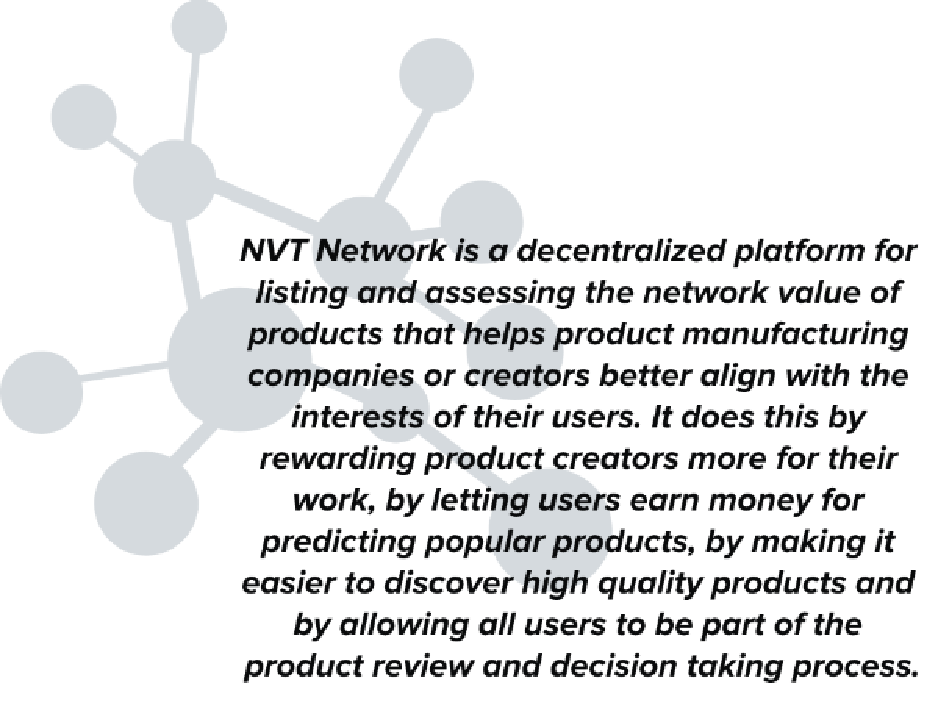
\includegraphics[scale=0.7]{Figures/nvt-desc}
\end{figure}
\vfill
% {\large \today}\\[4cm] % Date
% 
\includegraphics{Figures/nvt-network-logo-eps-v1} % University/department logo - uncomment to place it
 
\vfill
\end{center}
\end{titlepage}

%----------------------------------------------------------------------------------------
%	ABSTRACT PAGE
%----------------------------------------------------------------------------------------

\begin{abstract}
\addchaptertocentry{\abstractname} % Add the abstract to the table of contents
The \textit{Network Value Token (NVT Network)} is a decentralized platform for listing and assessing product network value, with its aim being to align manufacturer interests with those of their users. In this way, we cultivate a mutually beneficial relationship between the two parties. This is accomplished by (1) promoting manufacturer rewards, (2) rewarding user predictions, (3) streamlining the product-discovery pipeline and (4) staking a fair and equal share of the product decision-making process to each network user. Overlaying the \textit{NVT Network} on the surface level is the \textit{NVT Community}, a novel online information community for product reviewing. The \textit{NVT Community} consists of four user types: (a) Creators, (b) Explorers, (c) Moderators and (d) Product Users. The \textit{NVT Network} forms the basis for a product-based prediction market, where market metrics are derived from product network value. We construct a robust pricing system which incentivizes users to discover and share products within the network, allowing the best content to rise to the top of the \textit{NVT Community}. What fuels the \textit{NVT Network}, which we keep open and accessible to all users, is the \textit{NVT Token}. The network rewards \textit{NVT Tokens} for user contributions, making it a network participation a net benefit for everyone.The \textit{NVT Community} is deployed on \textit{NVT Network's} native blockchain, guaranteeing which accessibility, performance, transparency, and speed. For the first time in the technology sector, the \textit{NVT Network} implements a decentralized, user-generated product-review ecosystem, one driven by both fairness and quality.
\end{abstract}

%----------------------------------------------------------------------------------------
%	ACKNOWLEDGEMENTS
%----------------------------------------------------------------------------------------

\begin{acknowledgements}
\addchaptertocentry{\acknowledgementname} % Add the acknowledgements to the table of contents
NOTHING IN THIS WHITEPAPER CONSTITUTES LEGAL, FINANCIAL, BUSINESS OR TAX ADVICE. YOU SHOULD CONSULT YOUR OWN LEGAL, FINANCIAL, TAX OR OTHER PROFESSIONAL ADVISER(S) BEFORE ENGAGING IN ANY ACTIVITY IN CONNECTION HEREWITH. NEITHER THE NVT FOUNDATION (THE FOUNDATION), ANY OF THE PROJECT TEAM MEMBERS WHO HAVE WORKED ON NVT NETWORK (AS DEFINED HEREIN) OR PROJECT TO DEVELOP NVT NETWORK IN ANY WAY WHATSOEVER (THE NVT NETWORK TEAM), ANY DISTRIBUTOR/VENDOR OF NVT (THE DISTRIBUTOR), NOR ANY SERVICE PROVIDER SHALL BE LIABLE FOR ANY KIND OF DIRECT OR INDIRECT DAMAGE OR LOSS WHATSOEVER WHICH YOU MAY SUFFER IN CONNECTION WITH ACCESSING THIS WHITEPAPER, THE WEBSITE AT \url{https://nvtnetwork.com} (THE WEBSITE) OR ANY OTHER WEBSITES OR MATERIALS PUBLISHED BY THE FOUNDATION.
\end{acknowledgements}

%----------------------------------------------------------------------------------------
%	LIST OF CONTENTS
%----------------------------------------------------------------------------------------

\tableofcontents % Prints the main table of contents

%----------------------------------------------------------------------------------------
%	THESIS CONTENT - CHAPTERS
%----------------------------------------------------------------------------------------

\mainmatter % Begin numeric (1,2,3...) page numbering

\pagestyle{thesis} % Return the page headers back to the "thesis" style

% Include the chapters of the thesis as separate files from the Chapters folder
% Uncomment the lines as you write the chapters

% Chapter 1

\chapter{Introduction} % Main chapter title

\label{Chapter1} % For referencing the chapter elsewhere, use \ref{Chapter1} 

Over the last few years, distributed ledger technology and trustless blockchain have begun to rewire the state of communication, knowledge, and the entire economy. In particular, such technology has the potential to transform the financial services industry, benefiting both clients and participating firms alike. Distributed ledgers promise a future where every agreement is automatically recorded and managed without error, making sure anyone can make frictionless transactions for any contractual purpose. Phenomena such as duplication, reconciliation, failed matches, and breaks will all be a relic of the past. The combined success of the free software ecosystems, decentralized file-sharing, and public cryptocurrencies has rekindled the notion that decentralized internet protocols can radically improve societal infrastructure.

Redundant products overwhelm us all in the information era; judging product authenticity is more difficult than ever before. This creates a harsh environment for product discovery, resulting in the loss of many otherwise valuable products. Rather than worrying about product scarcity, consumers are exhausted by the barrage of goods and services made available to them. This problem - the inefficiency inherent to uncovering valuable information - is, unfortunately, central to the current market in the information era. 
A value network is a set of connections between organizations, corporations, and people, in which each of the three entities interact with each other for the benefit of the entire network. Such a network allows its members to buy, sell, and share information. The advantage of said network comes from the manner in which an entity applies the resources, influences and insights of others in the network. By combining utility and fairness, \textit{NVT Network}, our community-driven blockchain platform, not only ensures that high quality products stand out, but that quality product creators are rewarded accordingly.


%----------------------------------------------------------------------------------------

% Define some commands to keep the formatting separated from the content 
\newcommand{\keyword}[1]{\textbf{#1}}
\newcommand{\tabhead}[1]{\textbf{#1}}
\newcommand{\code}[1]{\texttt{#1}}
\newcommand{\file}[1]{\texttt{\bfseries#1}}
\newcommand{\option}[1]{\texttt{\itshape#1}}

%----------------------------------------------------------------------------------------

\section{Product Value}

Traditionally, markets have measured product value in terms of revenue. Product revenue is, in turn, influenced by the broader product market, i.e. products are interdependent. Such influence is particularly evident in the e-commerce sector, where websites present products through a collection of web pages linked by recommendation hyperlinks. This creates a large-scale product network. Better metrics for product value can help brand or category managers recognize what to offer (or stop offering) on their site to customers, what to market more heavily, and how to better calculate prices. Such a network is invaluable to advertising strategies, too, e.g. in influencing advertisers’ bidding behavior in pay-per-click (PPC) environments.

Traditionally, marketers have assessed the value of a product or brand according to the direct revenues the product creates, for example, based on the expected discounted cash flow in measurement methods such as that used by Interbrand. Yet the true value generated by a product that is part of a network, labeled as ”network value”, should take cross product effects into account. Specifically, it should consider both the revenues an item generates by directing traffic to other items and the revenues an item is not ”entitled” to due to traffic directed to it by other items.

In this whitepaper, we propose a method for assessing the network value of items in a large scale product network, using an approach that combines Google's \textit{PageRank} algorithm for assessing the popularity of web pages together with decentralized community user data.

The revenue of each product in the network, or each node, is derived from intrinsic and incoming value. Intrinsic value is self-generated by the item and incorporates retailer marketing activity. Incoming value is driven by incoming recommendation links, or edges of the network, pointing from other products to the product in question. It is assumed that the incoming value of a given product ”belongs” to the items that point to that product, rather than to the product itself. Thus, a product’s network value is defined (i.e., the value that takes into account its network relationship) as the sum of its intrinsic value and the value it generates for its neighbors through its outgoing links. We label this latter value as its outgoing value.

%----------------------------------------------------------------------------------------

\section{The Search for Product Quality}

The price of a product is an important indicator of its quality. This indicator can be used in the proposed model, derived by economic principles, in order to construct a prediction and review market for products. This idea is derived from the efficient markets hypothesis. The efficient market was first introduced by Bachelier, who recognized the efficiency of the market in selecting information. The discountings of past, present, and future events have their reflections in the prices of the market.

It is assumed that the investors in the market have access to independent analysis of the value of each item. Furthermore, they are considered rational, aiming at maximizing their own profits. Therefore, it’s practical to use the wisdom of the crowd to set a price for each product, where the price is a close prediction of the true value of the product.

\section{A Network-Based Product Prediction Market}

A prediction market is a platform where people trade based on event outcomes. Profit comes from making a correct prediction. Reward distribution for these predictions follows a simple, yet effective, principle: transfer profits from wrong predictors to right predictors. With these rewards in mind, analysts optimize as much as possible for logical and accurate predictions, derived from the best methods and information that they can find.

The proposed methodology for building NVT's prediction market follows a simple but effective idea (Eq. (1.1)). Users can rate a product, and if a user thinks the current prediction price of a product is lower than the actual value, he can upvote said product to raise the price. The cost of upvoting, or boosting, goes to the price increase of the product. If the final price gets higher than the predicted price, the user is rewarded within the NVT Network.

\begin{equation}
	\textrm{New Price} = \textrm{Current Price} + \frac{\textrm{Cost of Boost}}{\textrm{Upvote}}
\end{equation}

\section{Network Effects}

Network effects become significant after a certain subscription percentage has been achieved, called critical mass. At the critical mass point, the value obtained from the good or service is greater than or equal to the price paid for the good or service. As the value of the good is determined by the user base, this implies that after a certain number of people have subscribed to the service or purchased the good, additional people will subscribe to the service or purchase the good due to the value exceeding the price.

A key business concern must then be how to attract users prior to reaching critical mass. One way is to rely on extrinsic motivation, such as a payment, a fee waiver, or a request for friends to sign up. A more natural strategy is to build a system that has enough value without network effects, at least to early adopters. Then, as the number of users increases, the system becomes even more valuable and is able to attract a wider user base. Network effect relates to the intellectual commons in a positive way.

Through P2P networks users are able to share their intellectual property in a way that can benefit society as a whole. The sharing of intellectual property ultimately relates to economic growth due to the ability for creators to share information and still possibly benefit financially from it. Additionally, people are able to share types of education like scholarly articles, becoming a new form of public commons.

Network externality like Ted.com is an example of how intellectual commons benefit society as a whole. Those who present intellectual property at Ted conferences are sharing their education on a public forum that benefits whoever will listen. Therefore, the larger Ted.com network becomes positively correlates to those who benefit from its common-pool resources. The reward for being part of a group, society, and even the world through a P2P network is one of the greatest benefits that a modern common-pool resource can provide. The ability to connect and create with people from different cultures, ethnicities, and beliefs is something thought to be impossible a few years ago. Without network externality this form of communication would have been impossible.

\section{Blockchain}
\subsection{Evolution}

Public blockchains have emerged as a plausible messaging substrate for applications that require highly reliable communication. Bitcoin represents the first generation of blockchain, which has started the crypto revolution in the world. The second generation of blockchain technology is led by Ethereum. Ethereum allowed for the creation of smart contracts which made blockchain allow not only cash like tokens but also financial instruments like loans and bonds.

An important breakthrough of blockchain is ”Proof of Stake (PoS)”. Most ledgers nowadays are secured by ”Proof of Work (PoW)”, which require significant amount of processing power and thus electricity. In comparison, the PoS systems assign the block rewards to token holders proportionally, which significantly reduce the processing power and amount of energy needed in order to mine a block and is much more power efficient.

\subsection{Security as a Primary Factor}
 
Blockchain as a transnational platform, has security as its first priority. It is as the name implies, a chain of digitally connected data blocks. Blockchain was created in order to provide means of security by allowing for the existence of a decentralized ledger. Even though blockchain has many security properties, there still exist vulnerabilities and malicious attacks that need to be considered.

Blockchains are decentralized across peer-to-peer (P2P) networks that need to stay up to date and in sync with a consensus algorithm (e.g. PoW or PoS). A PoW based blockchain would require at least 51 per cent hash power of the network to perform a double-spend attack that could revert transactions. An attack like that highly depends on how decentralized the network is, as decentralization always makes it harder for attackers to succeed.

\subsection{Blockchain Interoperability}

Blockchain interoperability is the ability to transfer information from one blockchain to another. Today there are hundreds of blockchain networks entirely disconnected from each other, leading to inefficiency. This lack of communication makes it difficult for the blockchain technology to truly scale and allow its users to enjoy the full potential. Furthermore, interoperability can also improve the efficiency of the markets, allowing for much faster transactions between different protocols and services.

\subsection{Hyperledger}

The Hyperledger Project is a collaborative effort to define and develop industrystandard blockchain technology that can be used by developers to build applications for multiple industries. It is an open-source project hosted by the Linux Foundation, which is home to many other open-source initiatives including the widely used Linux operating system.

The Hyperledger Project works like most other open-source projects; various companies contribute software code, and the contributions are reviewed, combined and further developed to create the software ultimately released by the Project. Companies that have contributed software include IBM, Digital Asset Holdings (DAH) and financial-software consortium R3. DAH is a financial-software company that also contributed the Hyperledger name, which it previously owned. R3 provided a distributed ledger designed for financial transactions.

Hyperledger currently has close to 100 members and more than 100 contributors. Under the umbrella of the Hyperledger Project are several individual software development projects, all of which are at an early ”incubation” stage. The Hyperledger Fabric project focuses on core blockchain technology, including support for smart contracts, and is designed to act as a foundation for developing blockchain applications or solutions.

\subsection{Interledger}

Interledger is not a distributed ledger project per se. Instead, it focuses on connecting different ledgers. The project centers on the Interledger Protocol (ILP), which is designed to enable communication between different international payment systems around the world. The idea is that any payer should be able to pay any payee, quickly and at little or no cost, without the need for both parties to set up accounts on the same global payment service.

\subsection{Scalability}

One approach to the scalability issues is by splitting up different transactions across multiple different blockchains. While this lowers the transactional demand on any blockchain used, the hash pool power will be just as low. With smaller networks on each blockchain, it is easier for someone to take over enough hash power in order to perform a double spend attack. While it offers some degree of scalability, security is considerably lower and it is definitely not a long-term solution. Multiple blockchains also limit cross chain transactions to exchanges that charge additional trading fees, have long processing times and often security issues.

\subsection{Lightning Network}

Lightning Network is a ”second layer” payment protocol that operates on top of a blockchain (most commonly Bitcoin). It enables instant transactions between participating nodes and has been touted as a solution to the Bitcoin scalability problem. It features a peer-to-peer system for making micro-payments of digital cryptocurrency through a network of bidirectional payment channels without delegating custody of funds and minimizing trust of third parties.

Normal use of the Lightning Network consists of opening a payment channel by committing a funding transaction to the relevant blockchain, followed by making any number of Lightning transactions that update the tentative distribution of the channel’s funds without broadcasting to the blockchain, optionally followed by closing the payment channel by broadcasting the final version of the transaction to distribute the channel’s funds.

\subsection{Proof of Work (POW)}

This is the most popular algorithm being used by currencies such as Bitcoin and (at the time of writing) Ethereum, each one with its own differences. In PoW, in order for an actor to be elected as a leader and choose the next block to be added to the blockchain they have to find a solution to a particular mathematical problem. Given that the hash function used is cryptographically secure, the only way to find a solution to that problem is by brute force (trying all possible combinations). In other words, the actor who will solve the aforementioned problem first the majority of the time is the one who has access to the most computing power. These actors are also called miners. It has been widely successful primarily due to its following properties:

\begin{enumerate}
\item It is hard to find a solution to that given problem.
\item When given a solution to that problem it is easy to verify that it is correct.
\end{enumerate}

Whenever a new block is mined, that miner gets rewarded with some currency (block reward, transaction fees) and thus are incentivized to keep mining. In PoW, other nodes verify the validity of the block by checking that the hash of the data of the block is less than a preset number. Due to the limited supply of computational power, miners are also incentivized not to cheat. Attacking the network would cost a lot because of the high cost of hardware, energy, and potential mining profits missed.

\subsection{Proof of Stake (POS)}

PoS takes away the energy and computational power requirement of PoW and replaces it with stake. Stake is referred to as an amount of crypto currency an actor is willing to lock up for a certain amount of time. In return, they get a chance proportional to their stake to be the next leader and select the next block.

The main issue with PoS is the so called ”nothing at stake” problem. Essentially, in the case of a fork, stakers are not disincentivized from staking in both chains, and the danger of double spending problems increase. In order to avoid that, hybrids consensus algorithms appeared, such as the PoW-PoS combination. Active research towards a secure and decentralized PoS protocol is being done by the Ethereum Foundation with Casper The Friendly Ghost and Casper The Friendly Finality Gadget.

%----------------------------------------------------------------------------------------

\section{Ethereum}

Ethereum is a decentralized platform that runs smart contracts: applications that run exactly as programmed without any possibility of downtime, censorship, fraud or third-party interference. These apps run on a custom built blockchain, an enormously powerful shared global infrastructure that can move value around and represent the ownership of property. This enables developers to create markets, store registries of debts or promises, move funds in accordance with instructions given long in the past (like a will or a futures contract) and many other things that have not been invented yet, all without a middleman or counterparty risk.

Ether is a necessary element; fuel for operating the distributed application platform Ethereum. It is a form of payment made by the clients of the platform to the machines executing the requested operations. Ether is the incentive ensuring that developers write quality applications (wasteful code costs more) and that the network remains healthy (people are compensated for their contributed resources).

\subsection{A Decentralized Network}

On traditional server architectures, every application has to set up its own servers that run their own code in isolated silos, making sharing of data hard. If a single app is compromised or goes offline, many users and other apps are affected. On a blockchain, anyone can set up a node that replicates the necessary data for all nodes to reach an agreement and be compensated by users and app developers. This allows user data to remain private and apps to be decentralized like the Internet was supposed to work.

\subsection{ERC20}

ERC20 is a technical standard used for smart contracts on the Ethereum blockchain for implementing tokens. ERC20 defines a common list of rules for Ethereum tokens to follow within the larger Ethereum ecosystem, allowing developers to accurately predict interaction between tokens. These rules include how the tokens are transferred between addresses and how data within each token is accessed.

% Chapter Template

\chapter{Problem Statement} % Main chapter title

\label{Chapter2} % Change X to a consecutive number; for referencing this chapter elsewhere, use \ref{ChapterX}

Ad-driven models fall prey to serving the needs of advertisers and looking things through their scope. Most online content review platforms do not distribute value to their creators and users with fairness in mind. Some of the existing platforms have tried to solve these problems with crypto monetization and extra rewards to the creators and users. While this is an interesting approach, their discovery mechanisms can be easily manipulated by bots. The proposed concept of NVT Network, is trying to revolutionize the online reviewing industry by launching a solution that solves the following problems:

\begin{enumerate}
\item Unequal Distribution and Platform Value.

Users are contributing content and data to online platforms, but these platforms are capturing an unequal amount of the value created by users' content. Creators and users deserve to be rewarded more efficiently for the services they provide or data they contribute to an online network. Blockchain networks like NVT, provide a new way to share network value more fairly to everyone.

\item Ineffective Product Discovery.

People need a reliable way to find quality services and products. Old and out of date platforms, which are promoting creators and their products, have issues with manipulation and paid upvoting bots that harm content ranking quality, review and board spamming. This makes it hard for users to quickly find good quality services.

\item Centralized Product Review Moderation.

Moderators are an important part of online communities as they decide which listings should get listed on the platform, monitor the actions of the users and apply penalties if needed, influence and moderate content promotion, etc. This centralized control means that other users do not have a formal way to dispute decisions made by moderators. NVT Network is exploring ways to change this.

\end{enumerate}

%----------------------------------------------------------------------------------------
%	SECTION 1
%----------------------------------------------------------------------------------------

\section{Type of Value}
\subsection{Tangible Value}

All exchanges including goods, services or revenues and transactions are considered tangible values. The transactions might involve contracts, invoices, request for proposals or confirmations, return receipts of orders and payments. Products or services that are expected to generate revenue are also included in the tangible value flow. In government agencies these would be mandated activities. In civil society organizations these would be formal commitments to provide resources or services.

%-----------------------------------
%	SUBSECTION 1
%-----------------------------------
\subsection{Intangible Value}

Two primary subcategories are included in intangible value: knowledge and benefits. Intangible knowledge exchanges include strategic information, planning knowledge, process knowledge, technical know-how, collaborative design and policy development; which support the product and service tangible value network. Intangible benefits are also considered favors that can be offered from one person to another. Examples include offering political or emotional support to someone. Another example of intangible value is when a research organization asks someone to volunteer their time and expertise to a project in exchange for the intangible benefit of prestige by affiliation.

All biological organisms, including humans, function in a self-organizing mode internally and externally. That is, the elements in our bodies down to individual cells and DNA molecules work together in order to sustain us. However, there is no central ”boss” to control this dynamic activity. Our relationships with other individuals also progress through the same circular free flowing process as we search for outcomes that are best for our well-being. Under the right conditions these social exchanges can be extraordinarily altruistic. Conversely, they can also be quite self-centered and even violent. It all depends on the context of the immediate environment and the people involved.


%-----------------------------------
%	SUBSECTION 2
%-----------------------------------

\subsection{a Non-Linear Approach}
Often value networks are considered to consist of groups of companies working together to produce and transport a product to the customer. Relationships among customers of a single company are examples of how value networks can be found in any organization. Companies can link their customers together by direct methods like the telephone or indirect methods like combining customer’s resources together. The purpose of value networks is to create the most benefit for the people involved in the network. The intangible value of knowledge within these networks is just as important as a monetary value. In order to succeed, knowledge must be shared to create the best situations or opportunities. Value networks are how ideas flow into the market and to the people that need to hear them.

%----------------------------------------------------------------------------------------
%	SECTION 2
%----------------------------------------------------------------------------------------

\section{An Alternative to Mining}

Referring a friend or distributing knowledge and informational reviews about products, networks or groups to other social media channels, is essential to the community. These points can be used in promotion of a listing. Product-discovery can be compared to proof of work. Mining requires electricity, and the electricity bills in this case can be paid either by NVT tokens or labor for the growth of the community. The process of product-evaluation and the prediction model is described in Section 3.1.

The basic principle behind this idea is that any user can assign NVT tokens to creators, networks or listings according to the judgment and community review of the product. Additionally, any user can assign NVT tokens to the community and user or explorer base according to the foresight of each voter.

%----------------------------------------------------------------------------------------

\section{Core Transparency}

Because the number of fraudelent projects is too high, it can be hard for investors to decide which one is worthy and has legitimacy. The NVT Team believes that investors and token sale organizers alike, will benefit from some form of increased financial transparency. It will give the investors the confidence needed that a startup is directing the funds given toward the development of the project and its vision. Quality startups likely, attract more funds when properly demonstrate a wisely constructed financial plan to the investors.

This has led the NVT Team to decide that it is imperative to lock its tokens for a vesting period of 12 months. Furthermore, a special report page will be made at the \href{https://nvtnetwork.com/}{NVT Foundation Website}, including the addresses of everyone involved with the team and their wage transactions. Lastly, the NVT Team will always be available to community review and it is going to be transparent with its expenses and all other financial data.

%----------------------------------------------------------------------------------------

\section{Network Value Transactions}

In traditional finance, ratio analysis is one of the most widely used valuation methods. Lacking the detail of other valuation approaches, such as DCF analysis, ratio-based valuation is much faster and is still a good proxy of fair value. It also allows one to easily track asset price dynamic over long periods of time as well as compare different assets to each other. Over the course of the last year, a new study of cryptoeconomic ratio analysis emerged. One of the most widely known ratios is Network Value to Transactions, or NVT.

In a traditional PE ratio, the earnings metric in the denominator is used as a proxy for the underlying utility of the company created for the shareholders. While cryptoassets do not have earnings, one can argue that the total value of transactions flowing through the network is a proxy for how much utility users derive from the chain.

It is worth highlighting that Daily Transaction Volume in NVT takes into account only on-chain transactions. All the trading activity that happens on exchanges and is, for the most part, speculative is not included in this volume. Some researchers argue that NVT can be successfully used to detect bitcoin price bubbles when valuation is not supported by fundamentals and differentiate them from consolidations. If we analyze historical data, the spike in NVT follows the bubble with a considerable lag of a few months. Peak NVT coincides with the middle of a correction period. NVT is neither predictive (does not precede the overvaluation), nor descriptive (does not coincide with it). You can only detect the bubble a few months after it bursts.

We claim that this refined NVT ratio is a better descriptive metric of generic bubbles. Conceptually, this makes sense. Given that Transaction Volume in NVT is a proxy for fundamental utility value of the network, a 90-day Moving Average is a better proxy for long-term fundamental value than a 28-day Moving Average.

Let’s now look at the recent bitcoin price performance using the refined NVT ratio in more detail. From January until mid-December 2017, bitcoin has appreciated almost 20x. For the most part of this rally, though, NVT ratio has stayed in the Green Zone. However, in December when price reached almost \$20k, NVT went into the Yellow for a few days. This rapid appreciation was shortly followed by a 30\% price correction, and another even steeper price correction in the last weeks. After the correction, NVT has returned to the Green zone. This is another empiric evidence in support of 90 MA NVT.

There is, however, another more fundamental weakness of NVT. It only takes into account total value of on-chain transactions, but it does not factor in the number of transactions or the number of addresses (wallets) participating in these transactions. For internet companies, especially marketplaces, social networks, and other businesses with strong network effects, the analogous Daily Active Users (DAU) indicator is one of the most important performance and valuation metrics. This and other metrics that now make up the language of valuing internet companies did not exist in the 1990s. It has been developed by technology investors over the last 20+ years. Similar valuation framework for cryptoassets is yet to be developed and is only starting to form.

%----------------------------------------------------------------------------------------

\section{Solution and Benefits}
NVT Network is a prediction market and listing protocol that helps networks and creators better align with the quality of service they provide to users. This is accomplished by:

\begin{itemize}
\item A fair and efficient promotional system for creators and service providers.
\item User rewards for predicting quality products, services or networks. 
\item Simplifying the process of high quality discoveries.
\item Allowing all users to participate in content moderation and community decisions.
\end{itemize}

Users and communities can enjoy some benefits with NVT Network such as:

\begin{itemize}
\item Rewards for their effort and their work.
\item Rewards for discovering quality products and services.
\item Buying products or services in exchange for NVT tokens.
\item Explore high quality products more efficiently. 
\item Be part of content, data and governance moderation. 
\end{itemize}

From a high-level perspective, NVT Network has three key protocols that power these benefits:

\begin{itemize}
\item \textbf{Token Rewards Protocol.}

Solution to the unequal value distribution problem. A decentralized protocol for managing token rewards for quality work, to creators, users, and moderators while allowing and giving the incentive to users to spend tokens on the network.

\item \textbf{Product Pricing Protocol.}

Solution to the ineffective services and products discovery problem. A prediction and discovery market protocol for valuing, reviewing and rating services, products and networks.

\item \textbf{Community Protocol.}

Solution to the centralized moderation problem. The community protocol enables users to participate in content moderation and community decisions. Additionally, NVT Network is creating its own listing and sharing platform, NVT Community, to demonstrate and allow everyone to enjoy the benefits of NVT Network.

\end{itemize}

%----------------------------------------------------------------------------------------

\section{Information Discovery}

Based on the definition of ”Information”, the purpose of ”Information” is to eliminate uncertainty. Meanwhile the cost of getting information varies for different individuals. Facing complicated blockchain technology and booming blockchain currencies, regular investors are ”blinded” by the explosion of information. It is hard for one to get reliable information about a project with time-efficiency.

NVT Community solves the product-rating problem with the decentralized prediction market. Under this information filtering mechanism, quality products will stand out. NVT Community is powered by the blockchain, inheriting all the advantages of blockchain technology.

The developed payment system paved the ground for features like ”Paid Q\&A”, ”Paid Subscription”, ”Pay to message”, ”Pay to survey”, and ”Sending gift reward”. All those features encourage the distribution of valuable information, and paid information exchange. 
% Chapter Template

\chapter{Network Design} % Main chapter title

\label{Chapter3} % Change X to a consecutive number; for referencing this chapter elsewhere, use \ref{ChapterX}

NVT Network follows two crucial principles in building an efficient product value prediction market:

\begin{itemize}
\item In a regular efficient market, there is not such thing as a free lunch. One has to pay to gain. In NVT Community, in order to incentivize users to discover good quality content, boosters and reviewers will be rewarded with NVT Tokens. This is a ”game” in which a return is expected, thus it has to come with an initial cost to balance the expected return. Therefore, each boost will cost a given amount of NVT Tokens, to prevent BOT cheating or manipulation.
\item It is imperative to treat every user with justice and fairness in order to build a free and truly decentralized market. Each user of the community will be able to get proportional rewards according to their contributions. The same way as a start-up company assigns its initial stocks to the employees with each major contribution. Every form of ”labor” should be valued equally and just. Contributing time to create, discover and distribute product reviews and data should be valued equally as if one is contributing money. In some ways one could even argue that time is more valuable than money. Based on the principle of fairness, we need a consistent mechanism to reward those who are doing quality work. High-quality content tends to inspire others and results in further creation of more high-quality reviews and articles. Therefore, when users spend NVT Tokens to upvote or boost a product, the community needs to assign a reasonable portion of NVT Tokens to the product creator in order to reward their contributions. Similarly, product discoverer and explorer (Booster) should also be rewarded for accurately finding the true value of a product or listing. The community implements a mechanism that redistributes NVT Tokens from late voters to early voters. In this way early stage voters have a higher expected return of NVT.
\end{itemize}

%----------------------------------------------------------------------------------------
%	SECTION 1
%----------------------------------------------------------------------------------------

\section{Proof of Network}

By introducing Proof of Network (PoN), the goal is to create an efficient, completely decentralized and community-driven prediction market. When users discover that the current score of a product is lower than their prediction or their expected valuation, they can boost or vote in order to positively alter the score of that particular product or network group. Every boost will cost a small amount of NVT Tokens or influence points.

This way, users that choose to participate and positively contribute to the community, have a higher chance to earn rewards more often, leading the users to actively try to discover worthy products, creators and deliver quality reviews.

%-----------------------------------
%	SUBSECTION 1
%-----------------------------------
\section{Product and Network Ranking}

NVT Community supports the creation of a community-driven and decentralized network value prediction market to make quality products stand out. Each stream or commit of information must be ranked based on the time that the post, the vote or the review was issued. The weight of each vote is calculated by taking the logarithm of total positive votes, adding it with the deposited NVT Tokens.

NVT Community users can enjoy additional rights by purchasing NVT Tokens and by locking them on the platform. Only locked NVT Tokens are added to the extra voting power. By reducing the liquidity of NVT Tokens with the locking function, the stakeholders’ interests are tied with the community. This way, the users are encouraged to implement judicious planning schemes, for their own self-interest.

Arbitrary votes would jeopardize the utility and community effect of the platform, therefore NVT Token stakeholders are more likely to make prudent judgment. Enhanced voting power for product, network and listings ranking is only fair for this occasion. Meanwhile, the logarithm operation prevents major stakeholders from having unchecked dictating powers. The voting weight for a popular post is inversely proportional to the rank of voters.

%-----------------------------------
%	SUBSECTION 2
%-----------------------------------

\section{Community Ecosystem}

NVT Community is composed of regular users, product creators, explorers and community moderators. Regular users can receive influence points by completing a given set of tasks. They can also be promoted to community ambassadors by contributing to the community. Users can be promoted to explorers by discovering quality products, networks and topics. They can also be elected as community moderators.

Explorers and content creators are considered core members in the development of the community. They will receive NVT Tokens as rewards for their contributed discoveries and posts. Network explorers can vote for topics and products in order to discover quality material for the community. Users can also vote for the highest performance contributing users so they can get extra NVT Tokens as rewards.

%----------------------------------------------------------------------------------------
%	SECTION 2
%----------------------------------------------------------------------------------------

\section{User Moderation}

Community moderators are elected every few weeks from regular users. The probability of a user being selected is proportional to the NVT Tokens one is staking on the platform. When someone gets elected as moderator by the community, it will result in NVT Token rewards. Community moderators ensure that the NVT Community is operating smoothly without problems and have some extra privileges when determining some future movements or decisions for the community.

One of the access levels of moderators, is the ability to delete questionable topics. To prevent abuse of such power, authors of removed content can appeal to the community. The appeal request would require a significant amount of NVT Token deposit. Users in the community can vote on the incident. Each vote would cost a small amount of NVT Tokens in order to prevent manipulation. After the appeal period has ended, if more than half of participants supports the notion, the appeal initiator would lose the deposit of NVT Tokens and the users who supported the appeal would also lose their NVT Tokens spent in the voting process. The same applies in the case of moderators losing the case vice-versa.

%----------------------------------------------------------------------------------------

\section{Community Rank}

The approach that is presented here is applicable to large scale decentralized databases which will be incorporated in the NVT Network. It can be implemented relatively straightforwardly, relying on observable data in comparison with input data from the community. This is of notable importance given that a product’s value is of interest not only to the retailer but also to external parties.

Intuitively, NVT Community Rank is based on a simple model of behavior: a consumer who ”browses” the community network randomly follows any one of the links on a page with equal probability. The algorithm is computed interactively and thus takes into account the effect of the entire network on each post, group or network. Mathematically, in each iteration, the algorithm divides a page’s Community Rank evenly among its successors (i.e., the pages it links to) in the network. Thus, the ranking of a page is ultimately the stationary probability that a random user who begins at a random page will visit the specific page.

Therefore, a page can gain a high community ranking by having either many pages or a few highly ranked pages that point to it. Although it is widely used as a measure of a node’s importance to a network, fundamentally, NVT Community Rank provides a proxy for the extent to which the network directs traffic to the node in question. NVT Rank can therefore be used as a benchmark value for the effect of the network on the traffic to a product’s page (and thus its demand).

%----------------------------------------------------------------------------------------

\section{Appeal System}

After the first appeal period ends, there is a cool-down timeframe in which if either the appeal initiator or the community moderator is unsatisfied by the result they can can start a second round of appeal. Next appeal will require exponentially more deposit than the previous one.

If the latest appeal is different from the previous one, the reward allocation for the previous one is voided and the final rewards are allocated based on the latest appeal result. This process is repeated until both party reach an agreement or either one is unwilling or unable to put down appeal deposit.

Community moderators will automatically assign a part of the NVT Tokens to users supporting them. If the appeal system overturns the original deletion, those NVT Tokens will be rewarded to users who disapproved of the deletion.

%----------------------------------------------------------------------------------------

\section{The Setting}

The revenue of a product is divided into two parts:

\begin{itemize}
\item The Intrinsic Value portion of the revenue is self generated by the item. It can be conceptualized as the revenue the product would be expected to yield on that website if it were not connected to others.
\item A product’s Incoming Value is driven by the recommendation links that point to that product from other products.
\end{itemize}

Thus, for product \textit{u}:

\begin{equation}
\textrm{Revenue(\textit{u})} = \textrm{IntrinsicValue(\textit{u})} + \textrm{IncomingValue(\textit{u})}
\end{equation}

We assume that an item’s Total Value consists of the product’s Intrinsic Value together with the product’s contribution to the Incoming Values of the products it recommends. The latter contribution is labeled as the ”Outgoing Value” of the focal product. We refer to the product’s total contribution to the firm (i.e., its Intrinsic Value together with its Outgoing Value) as its ”Network Value”:

\begin{equation}
\textrm{NetworkValue(\textit{u})} = \textrm{IntrinsicValue(\textit{u})} + \textrm{OutgoingValue(\textit{u})}
\end{equation}

This view is consistent with previous work assessing the value of customers in a network by distinguishing customers’ Intrinsic Value and the value they provide to the network.

%----------------------------------------------------------------------------------------

\section{PageRank as a Benchmark}

The goal of NVT Network is to develop an approach that will reallocate the value a product generates. It is suggested that this reallocation will be implemented according to the full recommendation system of the community group that the product is a part of.

Probably the best known computational tool that allows for a full network approach is PageRank, which is essentially an eigenvector centrality measure. This measure has been used for various applications involving ranking web pages. The best known application is Google’s ranking system, but PageRank has also been used for various academic research purposes, e.g. for understanding optimal advertising on the web.

The original PageRank algorithm provides a ranking of the importance of a web page in the hyperlinked structure of the web based on the following model:

\begin{equation}
\textrm{PageRank(\textit{u})} = \sum_{v \epsilon \textrm{ln(\textit{u})}} \frac{\textrm{PageRank(\textit{v})}}{\textrm{Out(\textit{v})}}
\end{equation}

where ln(\textit{u}) is the set of web pages (nodes) linking to node \textit{u} and Out(\textit{v}) is the number of outgoing links from node \textit{v}.

%----------------------------------------------------------------------------------------

\section{A Product Network Value Model}

The approach that is used to determine the network value of a product is similar to PageRank, with a fundamental difference. In sharp contrast with the existing methodology which considers only the traffic (value) that a product receives, in this work the traffic a product creates for other products is also considered.

Furthermore, similar to PageRank, different links (recommendations) generate different levels of traffic; thus, it is not enough to simply evaluate numbers of links. For example, in the context of Amazon, a link from Dan Brown’s best seller The Da Vinci Code is likely to be a more fruitful recommendation compared with one from a lower selling book.

The variable Impressions(\textit{v}) is defined as the number of people visiting product \textit{v}’s page (also frequently referred to as ”page views”) and observe its outgoing links. It is evident that not every link exposure leads to a purchase. Therefore, the recommendation conversion rate (RCR) associated with the product dyad (\textit{v},\textit{u}) is defined. RCR represents the probability that exposure to a link on \textit{v}’s page will result in a purchase of \textit{u}.

This probability is a combination of the probability that a link will be clicked on (frequently referred to as ”click through rate”) and the probability that the user’s visit to the next page will result in a purchase. Essentially, the RCR can be thought of as a ”cross selling conversion rate”.

We therefore define \textit{$a_{v \rightarrow u}$} an as the recommendation conversion rate (RCR) associated with the product dyad (\textit{v},\textit{u}); this RCR represents the probability that exposure to a link on \textit{v}’s page will result in a purchase of u. This probability is a combination of the probability that a link will be clicked on (frequently referred to as ”click through rate”) and the probability that the user’s visit to the next page will result in a purchase. Essentially, the RCR can be thought of as a ”cross selling conversion rate.

We can now define the Incoming Value of a product, that is, the sales that are attributed back to other products in the network, as:

\begin{equation}
\textrm{IncomingValue(\textit{u})} = \sum_{v \epsilon \textrm{ln(\textit{u})}} a_{v \rightarrow u} \times \textrm{Impressions(\textit{v})} \times P(u)
\end{equation}
where \textit{P(u)} is the price of product \textit{u}.

Note that the greater the volume of traffic directed to the product from neighboring products (i.e., the greater the number of Impressions of its neighbors or the links RCR), the larger the fraction of the product’s revenue that stems from its Incoming Value rather than its Intrinsic Value. For example, the Incoming Value of a book on Amazon that is recommended by many best sellers should be greater than that of a book that earns similar revenue despite not getting many recommendations or receiving recommendations from books that are not purchased often.

The remaining revenue generated by an item is by definition its Intrinsic Value (i.e., the revenue portion that is not generated by incoming links from other items in the network):

% \begin{equation}
% \textrm{IntrinsicValue(\textit{u})} = \textrm{Revenue(\textit{u})} - \textrm{IncomingValue(\textit{u})} = P(u) [ Q(u) - \sum_{v \epsilon \textrm{ln(\textit{u})}} a_{v \rightarrow u} \times \textrm{Impressions(\textit{v})}]
% \end{equation}

\begin{multline}
\textrm{IntrinsicValue(\textit{u})} = \textrm{Revenue(\textit{u})} - \textrm{IncomingValue(\textit{u})} \\ = P(u) [ Q(u) - \sum_{v \epsilon \textrm{ln(\textit{u})}} a_{v \rightarrow u} \times \textrm{Impressions(\textit{v})}]
\end{multline}

The outgoing value of item u is then the sum of all revenues that item u generates by recommending other products:

\begin{equation}
\textrm{OutgoingValue(\textit{u})} = \sum_{v \epsilon \textrm{Out(\textit{u})}} a_{u \rightarrow w} \times \textrm{Impressions(\textit{u})} \times P(w)
\end{equation}
where Out(\textit{u}) is the set of community group pages (nodes) to which node \textit{u} links.

Adding the Intrinsic Value of item \textit{u} to the product’s Outgoing Value, we obtain an expression for u’s Network Value:

% \begin{equation}
% \textrm{NetworkValue(\textit{u})} = \textrm{IntrinsicValue(\textit{u})} - \textrm{OutgoingValue(\textit{u})} = P(u) [ Q(u) - \sum_{v \epsilon \textrm{ln(\textit{u})}} a_{v \rightarrow u} \times \textrm{Impressions(\textit{v})}] + \sum_{v \epsilon \textrm{Out(\textit{u})}} a_{u \rightarrow w} \times \textrm{Impressions(\textit{u})} \times P(u)
% \end{equation

\begin{multline}
\textrm{NetworkValue(\textit{u})} = \textrm{IntrinsicValue(\textit{u})} - \textrm{OutgoingValue(\textit{u})} \\ = P(u) [ Q(u) - \sum_{v \epsilon \textrm{ln(\textit{u})}} a_{v \rightarrow u} \times \textrm{Impressions(\textit{v})}] \\ + \sum_{v \epsilon \textrm{Out(\textit{u})}} a_{u \rightarrow w} \times \textrm{Impressions(\textit{u})} \times P(u)
\end{multline}

where each product \textit{v} points to product \textit{u} and contributes to its incoming value, and product \textit{u}’s Outgoing Value stems from each product \textit{w} to which \textit{u} points. Note that a product cannot recommend itself and thus, by definition \textit{u} is unequal to \textit{v}.

% Figure 1: Sample Graph Containing Three Products
\begin{figure}[h]
\centering
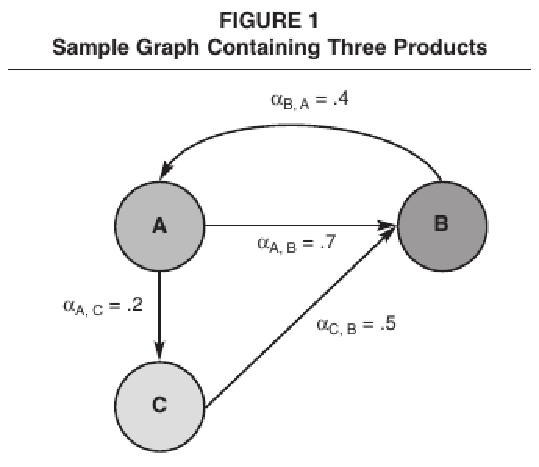
\includegraphics[]{Figures/figure_1}
\end{figure}

%----------------------------------------------------------------------------------------

\section{Quantifying Product Value}

A simple example is used to illustrate the application of the model. The definitions of the terms used are shown in Table 1. In Fig. 1, three linked products in an online e-commerce site are presented. RCRs and \textit{$a_{v \rightarrow u}$} are given and represent the probability that exposure to a link on \textit{v} will result in a purchase of \textit{u}.

Table 2 provides additional information on this small product network. For each Item (Column 1), the table presents the Quantity sold (Column 2), the Price per unit (Column 5), and consequently the total Revenue (Column 6).

The quantity of purchases of a product indicates the number of Impressions it receives (and thus recommendation exposure). However, Impressions can also stem from people who look at the product but do not purchase it. To move from Quantity

\begin{table}[ht]
\centering
\caption{Definitions}
\scalebox{0.45}{
\begin{tabular}{ll}
\hline\hline
\textbf{Term} & \textbf{Definition} \\ [0.5ex]
\hline
In(\textit{u}) & The set of web pages (nodes) linking to node \textit{u}. \\
Out(\textit{v}) & The set of web pages (nodes) to which node \textit{v} links. \\
P(\textit{u}) & The price of product \textit{u}. \\
Demand(\textit{u}) & The number of units of product \textit{u} sold. \\
Revenue(\textit{u}) & The total revenue a book generates (price x units). \\
Impressions(\textit{v}) & The number of people visiting product \textit{v}'s page (also frequently referred to as page views). \\
\textit{$a_{v \rightarrow u}$} & The PCR associated with the dyad (\textit{v,u}), which represents the probability that a customer exposed to a link to product \textit{u} on \textit{v}'s page will purchase product \textit{u}. \\
IntrinsicValue(\textit{u}) & The portion of product \textit{u}'s revenue that is not generated by incoming links from other items in the network. \\
IncomingValue(\textit{u}) & The sales of product \textit{u} that have been attributed back to the network. \\
OutgoingValue(\textit{u}) & The contribution of product \textit{u} to the incoming values of the product it recommends. \\
NetworkValue(\textit{u}) & The augmented value generated by a product that is part of a network. The sum of the product's intrinsic value and the value it generates for its neighbors through its outgoing links. \\
\textit{$k_u$} & The percentage of eventual buyers who viewed book \textit{u} and purchased book \textit{u}. \\
\hline
\end{tabular}}
\label{table:definitions}
\end{table}

\begin{table}[ht]
\caption{Network Value Algorithm Example, Iteration 1}
\centering
\scalebox{0.49}{
\begin{tabular}{c c c c c c c c c c}
\textbf{Item} & \textbf{Quantity} & \textbf{Impressions} & \textbf{Classical Conversion Rate} & \textbf{Price (\$)} & \textbf{Revenue (\$)} & \textbf{Intrinsic Value (\$)} & \textbf{Incoming Value (\$)} & \textbf{Outgoing Value (\$)} & \textbf{Network Value (\$)} \\
\hline
A & 10 & 13.33 & .75 & 100 & 1,000.00 & 975.00 & 25.00 & 145.33 & 1,120.33 \\
B & 5 & 6.25 & .80 & 150 & 750.00 & 395.71 & 354.29 & 25.00 & 420.71 \\
C & 20 & 28.57 & .70 & 20 & 400.00 & 394.67 & 5.33 & 214.29 & 608.95 \\
Total & & & & & 2,150.00 & 1,765.38 & 384.62 & 384.62 & 2,150.00 \\
\hline
\end{tabular}}
\label{table:example}
\end{table}

to Impressions, we can use a variable that is often reported for different e-commerce web sites, called the Conversion Rate. Conversion Rate is the percentage of page visits that actually result in a purchase (to differentiate this number from the cross product RCR, we label it the ”Classical Conversion Rate”). Thus, to get to the number of Impressions (Column 3), we can divide the Quantity (Column 2) by the Classical Conversion Rate (Column 4).

To understand the full value of each product, we first compute the Intrinsic and Incoming Values of each product. These refer, respectively, to the portion of the revenue that is self generated by the item (Intrinsic) and the portion of the revenue driven by the recommendation links pointing from other items to the focal item (Incoming). These values are presented in Columns 6 and 7 of Table 2.

Using Eq. 5, the Incoming Value of product B is computed:

% \begin{equation}

% \end{equation}

\begin{multline}
\textrm{IncomingValue(\textit{B})} = \sum_{v \epsilon \textrm{ln(\textit{B})}} a_{v \rightarrow B} \times \textrm{Impressions(\textit{v})} \times P(B) \\ = .07 \times 13.33 \times \$150 + .05 \times 28.57 \times \$150 \\ = \$139.96 + \$214.28 = \$354.29
\end{multline}

Using Eq. 6, the Intrinsic Value of product B is computed:

\begin{equation}
\textrm{IntrinsicValue(\textit{B})} = \textrm{Revenue(\textit{B})} - \textrm{IncomingValue(\textit{B})} = \$750 - \$354.29 = \$395.71
\end{equation}

Note that product C is responsible for most of its own revenue (i.e., it has a high Intrinsic Value), whereas product B ”owes” almost half of its revenue to network traffic (i.e., it has a high Incoming Value).

The second step of our approach assigns the Incoming Value of each product back to its incoming links. For example, product B’s Incoming Value is \$354.29, which is assigned back to products A and C, in proportion to the strength of their recommendations. This results in \$139.97 being assigned to product A and \$214.28 being assigned to product C. Similarly, product A’s Incoming Value (\$25) is assigned back to B (its only incoming link), and product C’s Incoming Value (\$5.33) is assigned back to A (its only incoming link).

After assigning the Incoming Values back to the incoming links, we can compute the Outgoing Value of each product using Eq.(7). A product’s Outgoing Value is the sum of the Incoming Values that the focal product generates for its neighbors. Column 9 of Table 2 presents the Outgoing Value of each product. In our example, B was assigned product A’s Incoming Value, such that:

\begin{equation}
\textrm{OutgoingValue(\textit{B})} = \sum_{w \epsilon \textrm{Out(\textit{B})}} a_{B \rightarrow w} \times \textrm{Impressions(\textit{B})} \times P(w) = .04 \times 6.25 \times \$100 = \$25
\end{equation}

The last step is computing the Network Value of each product as the sum of its Intrinsic Value and its Outgoing Value, using Eq. 8. Column 10 of Table 2 presents the Network Value of each product. Note that the total Network Value over the entire network is equal to the total revenue. That is, our model simply redistributes the revenues among the products.

For product B the Network Value is:

\begin{equation}
\textrm{NetworkValue(\textit{B})} = \textrm{IntrinsicValue(\textit{B})} + \textrm{OutgoingValue(\textit{B})} = \$395.71 + \$25 = \$420.71
\end{equation}

Note that product C generates almost all its own revenues, and only 1.3\% of its revenues are generated by the community recommendation made by product A. Product B, in contrast, is very dependent on external recommendations, which generate 47.2\% of its revenue. After attributing the revenues back to the items that generated them, we observe that the revenue that product C generates by recommending other items is higher than 41\% of the revenue it generates through its own sales. Finally, note that the total Network Value of product C is much higher than its revenue.


%----------------------------------------------------------------------------------------

\section{Iterations and Convergence}

A fundamental question when exploring influence in networks is that of the ”ripple” effect: To what extent can we assume that the network value created by an item spreads in a contagion like way into the network, beyond the first degree of separation?

Take, for example, a product network in which item A recommends item B, which recommends item C, which recommends item D. Consider item B in that network. When applied once, the model attributes to item B a proportion of the revenue from sales of item C, and item A is attributed a proportion of the revenue from sales of item B. This assumes that the recommendation effect of an item stops at the books it recommends and no ripple effect process occurs.

However, the picture may be more complicated if there is some effect beyond the first degree of separation. Some of the revenue from sales of item C that is attributed to item B should actually be attributed backward to item A, which generated part of item B’s traffic to begin with. Indeed, B’s actual contribution to C’s revenue should be decreased by the proportion of A’s contribution to B. In the same manner, B has some part in C’s contribution to D’s revenue, in that some of C’s value comes from the incoming value driven by B. In other words, an item is entitled to a share of another item’s network value, not just its revenue.

It is important to note here that although theoretically we could envision effects that stretch deep inside the product network, we assume a strong decay across degrees of separation. This is consistent with findings from the community and social network literature that show that influence is locally bound, with some researchers suggesting three degrees of separation as the typical limit. It is also in line with findings that suggest that the average shopping basket on sites such as Amazon and Barnes \& Noble contains fewer than three items.

Consistent with previous research, influence decays across the network exponentially. With our approach, almost all the effect is confined to the decentralized community driven review network, and only a relatively small part travels through to higher degrees of separation.


%----------------------------------------------------------------------------------------

\section{Product Determinations}

Companies increasingly aim to optimize their product and brand portfolios by considering the value that each product generates and eliminating items that do not provide enough value. Given the possible discrepancy demonstrated between revenue and network value, firms should look beyond revenue when making such decisions. Note that this direction is similar to the transition in the customer management literature from viewing a customer’s value (and consequently the customer portfolio) as based solely on his or her purchases, to a broader view that also takes into account the customer’s effect on others through word of mouth.

% \begin{figure}[h]
%     \centering
%     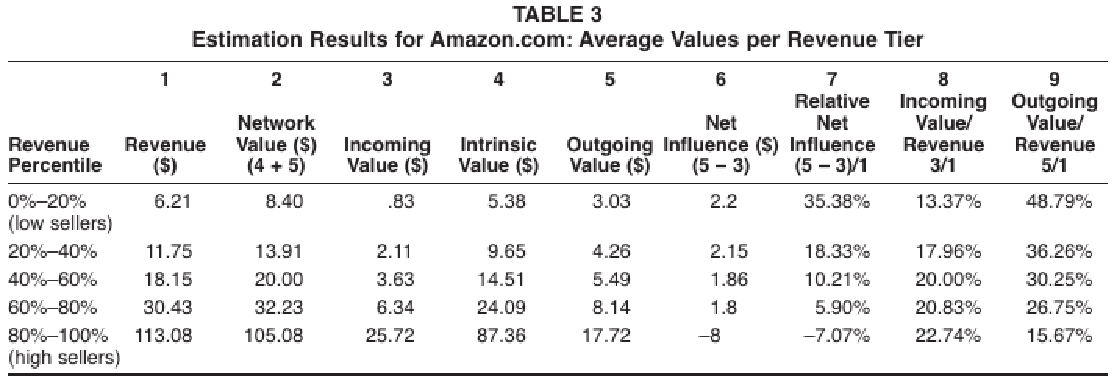
\includegraphics[width=\textwidth]{Figures/table_3.pdf}
% \end{figure}

The measure of the value to the firm created as a result of customers’ connectivity in the social network has been labeled customer referral value or customer social value. It should become of essential managerial importance as customers become more connected through tools such as social media and as marketers’ ability to follow

\begin{table}[ht]
\caption{Estimation Results for Amazon.com: Average Values per Revenue Tier}
\centering
\scalebox{0.32}{
\begin{tabular}{c c c c c c c c c c}
\textbf{Revenue Percentile} & \textbf{Revenue (\$)} & \textbf{Network Value (\$) (4+5)} & \textbf{Incoming Value (\$)} & \textbf{Intrinsic Value (\$)} & \textbf{Outgoing Value (\$)} & \textbf{Net Influence (\$) (5-3)} & \textbf{Relative Net Influence (5-3)/1} & \textbf{Incoming Value / Revenue 3/1} & \textbf{Outgoing Value / Revenue 5/1} \\
\hline
0\% - 20\% (low sellers) & 6.21 & 8.40 & .83 & 5.38 & 3.03 & 2.2 & 35.38\% & 13.37\% & 48.79\% \\
20\% - 40\% & 11.75 & 13.91 & 2.11 & 9.65 & 4.26 & 2.15 & 18.33\% & 17.96\% & 36.26\% \\
40\% - 60\% & 18.15 & 20.00 & 3.63 & 14.51 & 5.49 & 1.86 & 10.21\% & 20.00\% & 30.25\% \\
60\% - 80\% & 30.43 & 32.23 & 6.34 & 24.09 & 8.14 & 1.80 & 5.90\% & 20.83\% & 26.75\% \\
80\% - 100\% (high sellers) & 113.08 & 105.08 & 25.72 & 87.36 & 17.72 & -8 & -7.07\% & 22.74\% & 15.67\% \\
\hline
\end{tabular}}
\label{table:estimation}
\end{table}

this connectivity increases. Likewise, the ubiquity of decentralized product networks can make the network value of a product an important measure to help managers make informed product management decisions.

%----------------------------------------------------------------------------------------

\section{Product Network Influencers}

It is worthwhile to compare the results obtained regarding the ow of value in product networks with those obtained in research on social networks. Numerous studies have been devoted to the role of influencers and, in particular, hubs in social networks.

Who (or rather, which products) may be labeled ”influencers” in a product network? In most product networks, the number of outgoing links is limited, so a straightforward comparison to social network hubs is not trivial. More essential to the effect on others is the amount of traffic an item can send through its existing links, which we capture here in the number of impressions on the item’s page.

To connect influence to revenue tiers, we define influencers as the top 10\% in terms of outgoing value. The overall picture that emerges for the Amazon data is that the distribution of influence in the Amazon product network is spread across revenue tiers. Although the majority (56\%) of influencers are among the best sellers (top 20\% of revenue), the effect is still spread across other revenue tiers.

Another issue is that of net influence. Here, the comparison to social networks is limited, given that the research on the contribution of influencers in social networks has focused largely on the role of outgoing links, not incoming ones. If the influencers are defined as the group of products with the top 10\% of net influence, the best sellers are again most likely to be influencers. However in this case, they make up a smaller portion of the group (42\%), compared with influencers defined on the basis of outgoing value.

This result is particularly intriguing given that, on average, the net influence of this group is negative (see Table 3). Thus, it seems that there may be large differences among best sellers in terms of net influence, which are driven by incoming value.

%----------------------------------------------------------------------------------------

\section{Architectural Innovation and Performance Linkage}

Architectural innovation is described as an innovation that changed the way in which components of a product are linked together, while leaving the core design concept untouched. The core design concept explains the basic knowledge underlying the components. It destroys the usefulness of a firm’s architectural knowledge but preserves the usefulness of its knowledge about the product’s components.

In this description there is a distinction between the products as a whole (the entire system) and products in parts (components). The product as a whole explains how the components will work together. The components are defined as a distinct portion of the product that embodies a core design concept and performs a well defined function.

An example of an architectural innovation is the room air fan. The major components include the blade, the motor, the control system and the mechanical housing. The established technology is that of, large electrically powered fans, mounted in the ceiling. The introduction of a portable fan would be an architectural innovation. The primary components are largely the same, but the architecture of the product is quite different. There are also significant changes in the interactions between the components. For example the portable fan has a smaller size which means that there are new interactions between the motor size and the blade dimensions.

An architectural innovation draws attention to innovations that use many existing core design concepts in a new architecture and that therefore have a more significant impact on the relationships between components than on the technologies of the components themselves. The essence is to link existing components in a new way. The components themselves are not untouched. The central point is that the core design concept behind each component and the associated scientific and engineering knowledge remain the same. An architectural innovation is often triggered by a change in the components.

In the case of the room air fan the size is changed, that creates new interactions and linkages with other components in the established product. But it remains important that the core design concept behind the components stays the same.

%----------------------------------------------------------------------------------------

\section{Network Innovation}

A successful innovation depends on the spread of information and the exchange and combination of resources. Consequently the focus of innovation is found to be in networks and relations rather than in individual firms alone. Organizations build architectural knowledge around their relationships. Therefore communication channels, information filters and problem solving strategies play a significant role in architectural innovations.

An effective organization will organize itself around the product’s primary components in the network. These are the key relationships around which the organization builds architectural knowledge. An architectural innovation’s effect depends in a direct way on the nature of organizational learning about changes in architecture and about new interactions across components. The components are the key subtasks of the organization’s design problem.

%----------------------------------------------------------------------------------------

\section{Organizing Innovation}

How should the network be organized in order to improve the performance of an architectural innovation? It is argued that architectural innovation requires tight coordination across organizational boundaries. However it is unclear whether centralized, tight coordination by the innovation network’s leader improves architectural innovation. Next part will elaborate on the different influences of the level of betweenness on the innovation performance.

%----------------------------------------------------------------------------------------

\section{Network Decentralization}

The advantages and disadvantages of the level of betweenness within a network are elaborated. When should the lead firm organize innovation by using decentralized network approaches and when by using centralized network approaches? Centralized networks are those in which suppliers are tied to a ’lead’ firm. In decentralized networks suppliers have to meet the demands of diverse suppliers and customers by a market process or negotiation. Nobody in the network has total control.

The level of betweenness indicates the information control, it measures the centrality of a focal firm in a network and the extent to which a firm falls between pairs of other firms on the communication paths that link them. Betweenness is, in some sense, a measure of the influence a lead firm has over the information through the alliance network. The information control can be measured by the amount of network flow which is controlled by this firm.

Centralized or decentralized positions of a lead firm have different implications for innovations. The challenge for the lead firm is to choose the organizational form that matches the type of innovation they are pursuing the best. Why is a high level of betweenness (bureaucracy) bad, and a low level of betweenness (flexibility) good? Chesbrough and Teece (1996) argue that decentralized structures will be more responsive to a changing marketplace. This is because they are more flexible. Therefore, a decentralized innovation network can also play a more distinctive role in innovations. Most of their business is coordinated through the marketplace, resulting in more responsiveness than in case of a centralized lead firm. It is also argued that a decentralized approach is more efficient because not everything has to be reported to the lead firm. This ultimately saves time and money.

% Chapter Template

\chapter{Token Economics} % Main chapter title

\label{Chapter4} % Change X to a consecutive number; for referencing this chapter elsewhere, use \ref{ChapterX}

%----------------------------------------------------------------------------------------
%	SECTION 1
%----------------------------------------------------------------------------------------

\section{Properties and Usage of NVT}

The ERC-20 utility token of the NVT Network (NVT) is a major component of the NVT Network’s decentralized ecosystem. It is designed to be used solely as the primary token of the NVT Network. It is a non-refundable functional utility token that will be used as the unit of exchange between all users of the NVT Network.

NVT will provide a convenient and secure way of payment, reward and settling arrangements between users who explore and interact with the ecosystem of NVT Network. NVT does not in any way represent any shareholding, participation, right, title, or interest in the NVT foundation, its affiliates, or any other company, enterprise or undertaking, nor will NVT entitle token holders to any promise of fees, dividends, revenue, profits, or investment returns and are not indented to constitute securities in Singapore or any relevant jurisdiction.

NVT may only be utilized on the NVT Network and ownership of NVT carries no rights, express or implied other than the right to use NVT as a means to enable usage of and interaction with the NVT Network.

%-----------------------------------
%	SUBSECTION 1
%-----------------------------------
\section{Value Carrier}

NVT can be explained as the virtual crypto fuel of NVT Network, for using certain designed functions, services and tools of the decentralized platform. The economic incentives for users will encourage participants to contribute and take an active role in the decentralized community.

%-----------------------------------
%	SUBSECTION 2
%-----------------------------------

\section{Incentives}
Customer or membership incentive programs bring in new community members and reward existing members for their loyalty. A double-layer incentive mechanism based on the unique PoN (Proof of Network) algorithm is formulated on the platform and used to incentivize the users who contribute positively in the development of the community and ecosystem. In order to be fair to every user of the NVT Network, both creators and explorers will receive NVT as a reward.

Each user can vote for a product or network. There are two major sources of NVT rewards for product creators and explorers. One is user purchased NVT, the other is NVT converted from influence points for completing community and other contribution tasks. Those points are gradually released from the system’s reward pool. There is a limit on the weekly release so everything will be shared according to the pool of users and their performance. The reward pool will shrink every year, allowing for a better adoption rate at early stage. The platform will have a 5 per cent commission fee for the rewards assigned to users, in order to ensure the stability of NVT Network’s economic model.

%----------------------------------------------------------------------------------------
%	SECTION 2
%----------------------------------------------------------------------------------------

\section{Reward Setting}

The rewards that each user receives are always calculated accordingly to the order of the time someone sends the data or review during the early stage. The total number of users that participated in a vote, the time, the history and personal score of the user and other variables are taken under consideration during the process.

If a user discovers or predicts that a product will gain in popularity or user preference, the earlier he records his data, the more positive expected returns will receive as a reward for discovering worthy products early.

%----------------------------------------------------------------------------------------

\section{Bonus Malus}

Based on the system being fair, our community will be open and accessible for every user. Users participating will not be limited to those that have no earnings or points. Sharing, participating and being active on the community, will be few ways that someone will be able to get points.

To prevent fake user registration and bot attacks, we do not allow the exchanging of points with NVT Tokens. NVT Token is liquid and can be traded, also there will be limits on maximum points that can be earned. Users can use points for voting and decisions within the community. When points are used in the NVT Community prediction market, they can be converted to NVT Tokens.

%----------------------------------------------------------------------------------------

\section{Surveys and Prediction Market}

Within the NVT community there will be services and tools provided for users to create surveys and prediction requests for particular products, networks or assets. NVT Network will create products which will implement built-in decentralized prediction and assessment protocols. 
% Chapter Template

\chapter{Conclusion} % Main chapter title

\label{Chapter5} % Change X to a consecutive number; for referencing this chapter elsewhere, use \ref{ChapterX}

The increasing amount of research studying Internet recommendation systems is evidence of the increasing role of recommendation systems in consumers’ online shopping environments. Assessing the value of a product is crucial to informed marketing, including well planned advertising, brand portfolio planning, channel placement, cross selling initiatives, pricing, and compensation of marketing personnel. Understanding the network value of products is thus of essential importance for marketers.

In the early 90s, most web pages were created by academic institutions or magazines, and mostly contained plain text and hyperlinks to other sites. Over the next few years, the number of web pages grew exponentially, and online product retailers started to think about ways to expand. As the share of online purchases increases, the ability of firms to measure and affect network value will grow. Therefore, the NVT network should be a significant step toward a better understanding of this important concept. 

%----------------------------------------------------------------------------------------

\end{document}  
